\begin{prop}
    If $A \le G$, then $f(A) \le H$. In particular, Im $f = f(G) \le H$.
\end{prop}
\begin{propproof}
    $f(A)$ is non-empty since $e_H \in f(A)$.\\
    Let $x, y \in f(A)$, then $x=f(a_1), y=f(a_2)$, for $a_1, a_2 \in A$.\\
    We know $a_1a_2^{-1} \in A$, therefore, $f(a_1a_2^{-1}) \in f(A).$\\
    Now, $xy^{-1} = f(a_1)f(a_2)^{-1} = f(a_1)f(a_2^{-1}) = f(a_1a_2^{-1}) \in f(A).$\\
    According to subgroup criterion, $f(A) \le H$.
\end{propproof}
\begin{prop}
    Let $f^{-1}(B) = \{x \in G: f(x) \in B\}$. Then, if $B \le H$, then $f^{-1}(B) \le G$. Furthermore, if $B \lhd H$, then $f^{-1}(B) \lhd G$.
\end{prop}
\begin{propproof}
    \textbf{Part 1}\\
    We need to show that \( f^{-1}(B) \) is a subgroup of \( G \).\\
    Firstly, \( f^{-1}(B) \) is nonempty because $e_G \in f^{-1}(B).$\\
    Now, let \( x, y \in f^{-1}(B) \). Then \( f(x), f(y) \in B \). Since \( B \) is a subgroup of \( H \), $f(y)^{-1} \in B$, so:
    $$f(x) f(y)^{-1} = f(x) f(y^{-1}) = f(xy^{-1}) \in B.$$
    Thus, \( xy^{-1} \in f^{-1}(B) \), showing that \( f^{-1}(B) \le G\).\\
    \textbf{Part 2}\\
    We need to show that for all $g \in G$ and $x \in f^{-1}(B)$, $gxg^{-1} \in f^{-1}(B)$. \( x \in f^{-1}(B) \), so \( f(x) \in B \). Let's show $f(gxg^{-1}) \in B$.
    We have:
    \[
    f(gxg^{-1}) = f(g) f(x) f(g^{-1}) = f(g) f(x) f(g)^{-1}.
    \]
    Since \( f(x) \in B \) and \( B \) is normal in \( H \) (i.e., \( B \) is invariant under conjugation), we have:
    \[
    f(g) f(x) f(g)^{-1} = f(gxg^{-1})\in B.
    \]
    Thus, \( f(gxg^{-1}) \in B \), which implies \( gxg^{-1} \in f^{-1}(B) \).\\
    Hence, $f^{-1}(B) \lhd G$.
\end{propproof}
\section{Isomorphism Theorems}
\makebox[0pt][l]{%
\begin{tabular}{@{}m{0.65\textwidth}@{\hspace{1cm}}m{0.3\textwidth}@{}}
    {\small
    \textbf{Emmy Noether (1882–1935)} was one of most influential mathematicians of the 20th century known for her groundbreaking contributions in abstract algebra and theoretical physics. In 1927, she first introduced three isomorphism theorems (sometimes called Noether's isomorphism theorems) of group theory that generalize earlier ideas of abstract algebra. Noether's work exemplified abstraction and generalization. She moved mathematics away from computational techniques and concrete problems toward a more conceptual and unified framework. This approach is now a hallmark of pure mathematics.
    } &
    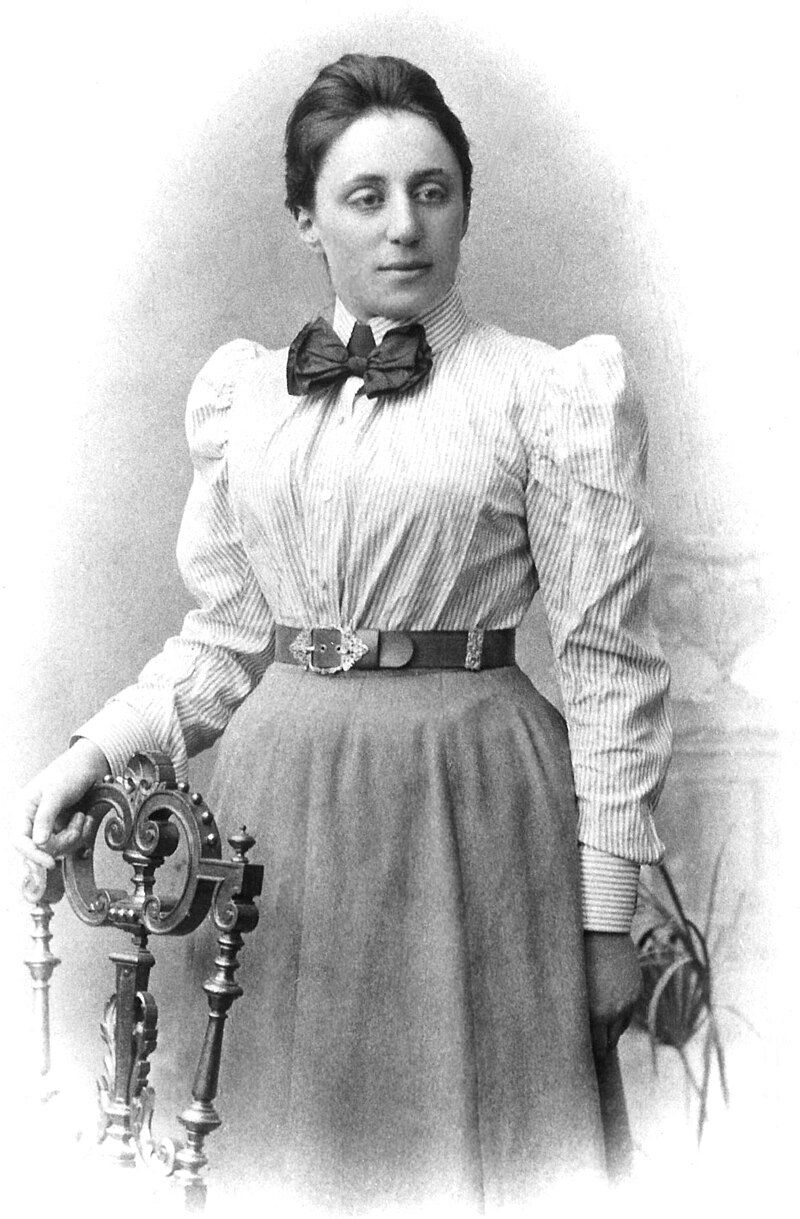
\includegraphics[width=\linewidth]{figures/Noether.jpg} 
\end{tabular}
}
\begin{theorem}[First Isomorphism Theorem]
    Let $f: G \rightarrow H$ be a group homomorphism. Then, there exits an injective homomorphism $f':G/\ker f \rightarrow H$ such that the following diagram commutes:
    \[
    \begin{tikzcd}
        G \arrow[r, "f"] \arrow[d, "\pi_{\ker f}"'] & H \\
        G / \ker f \arrow[ur, "f'"']
    \end{tikzcd}
    \]
    In particular, $G/\ker f \cong f(G)$.
\end{theorem}
\begin{proof}
    Let $N = \ker f$.\\
    $\pi_N: G \rightarrow G/N$.
    \begin{itemize}[label={}]
        \item \textbf{Define $f'$:} Let $f': G/N \rightarrow H$ such that $f'(aN) = f(a).$ The map is well-defined. Let $X \in G/N$. If $X = gN = g'N$, then $f'(X) = f'(gN) = f(g)$ and also $f'(X) = f'(g'N) = f(g')$. Since $gN = g'N$, it follows that $g = g'n$ for some $n \in N$. Using this, $f(g) = f(g'n) = f(g')f(n)$, and because $n \in \ker f$, we know $f(n) = e_H$. Therefore, $f(g) = f(g')$, so the map is well-defined.
        \item $f'$ is a \textbf{homomorphism:}
        \begin{align*}
            f'(aNbN) &= f'(abN)\\
                     &= f(ab)\\
                     &= f(a)f(b)\\
            \implies f'(aNbN) &= f'(aN) f'(bN)
        \end{align*}
        \item $f'$ \textbf{is injective}: By \hyperref[def:injectivehomo]{this} lemma, we know $f'$ is injective if and only if ker $f' = \{e_{G/N}\} = \{N\}.$ $f'(aN) = f(a) = e_H$ if and only if $a \in \ker f = N$.
        $$\ker f' = \{aN: a\in N\} = \{N\} = \{e_{G/N}\} $$
        Hence, $f'$ is injective.
        \item \textbf{The Diagram Commutes:} For all $g \in G, \pi_{\ker f}(g) = g \ker f$ and $f'(g \ker f) = f(g)$. Hence, $f = f' \circ \pi_{\ker f}$
        \item $f'(G/\ker f) = f(G)$. $f'$ is a homomorphism, $f'$ is injective and $f'$ is surjective onto it's image $f(G)$. Hence, $f'$ is bijective map from $G/\ker f$ to $f(G)$. Hence, $f'$ is an isomorphism from $G/\ker f$ to $f(G)$ which means $f'$ is an isomorphism from $G/\ker f$ to $f(G)$.
        Hence, $G/\ker f \cong f(G)$.
    \end{itemize}
\end{proof}